Typical DDMS workloads require large state, necessitating the use of more intelligent storage techniques.  However, compared to traditional DBMSes, DDMSes have more information to use when constructing a task-specific storage solution.  

These storage solutions consist of two primary components: (1) We can construct datastructures designed specifically for the DDMS' target query workload. (2) By analyzing the patterns with which data is accessed, we can identify a data layout strategy that reduces IO overhead.

\subsection{Datastructures}
Regardless of whether data is stored in memory, on disk, or across an entire cluster, efficient disk access begins with good representation.  We first consider one instance of a datastructure designed to efficiently support a DDMS' access patterns.  Data in the database can be categorized based on whether it is used in a selection predicate or group-by expression (a key column), or purely as data (a data column).  For example, consider example query $q$ from Section \ref{sec:dbtoaster}.  The column \texttt{extprice} is a data columns, while \texttt{sprior} and \texttt{ordkey} are examples of a key column.  

This clean categorization into key and data columns, suggests the use of key-value lookup datastructures, such as a hash-table.  However, the DDMS may perform lookups without specific values for all key columns; the datastructure should be able to provide an iterator over all key/value pairs that match a partially specified key.  Our primary concern is to provide lookup functionality for arbitrary subsets of the key columns, but one could extend this idea to employ range, nearest neighbor, and similar specialized indices.  

\comment{
Our first take on this key-value lookup structure, or \textit{map}, is a series of nested hash-tables, as shown in Figure \ref{fig:diag:nestedHash}.  Each level of nesting corresponds to a different key column.  Since there is typically no prefix ordering on keys used in the partial keys, we use secondary indices to support different orderings.
}

As one instantiation of this structure, Section \ref{sec:dbtoaster}'s $m_c$ would be stored not as a series of entries, but rather as two level nested hash table indexed by \texttt{custkey} and \texttt{ordkey} respectively.  Insertions into the \texttt{customer} table require an iteration over all values with \texttt{@ck = custkey}; the iterator loops over the inner hashmap.  Insertions into \texttt{lineitem} match on \texttt{@ok = orderkey} and require a secondary index.  

\comment{
\begin{figure}
\begin{center}
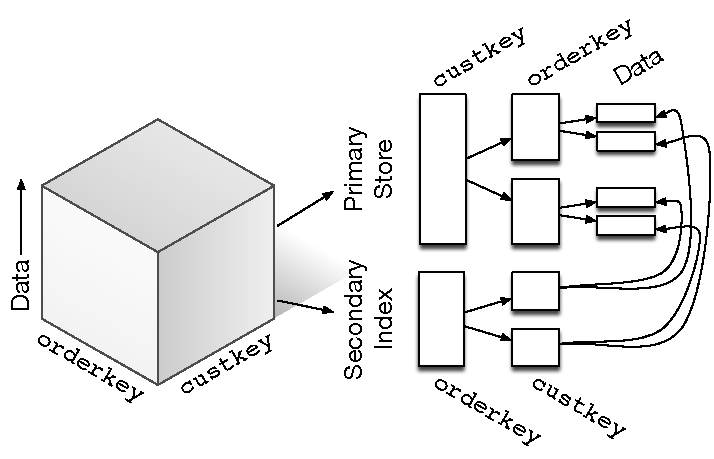
\includegraphics[width=2.5in]{graphics/MultikeyMap}
\end{center}
\caption{Expressing a multi-key iterable hash-table as a nested hash-table with secondary indices.  Secondary indices are optional, and only maintained for access patterns used by one of the DDMS' queries.}
\label{fig:diag:nestedHash}
\end{figure}
}

Initially, one might consider this a stale problem.  Systems with this sort of functionality\cite{berkeleydb} have been around for a while.  The critical insight however, is that the entire query workload is known in advance.  The DBToaster compiler can identify the \textit{complete} set of useful secondary indices \textit{at compile time}, including the potential benefits of more intricate indexing strategies like range queries\cite{rangequeries}.  Not only is this information useful at compile time, but it can be used to identify tradeoff points and generate a state machine for runtime index and layout tuning.

%%%%%% should we make any comments here about the relationship between the presence of secondary indices and partitioning schemes?  Otherwise, I'm not sure we have anything to say about maps and datastructures other than (like tables) they're very amenable to horizontal partitioning.

\subsection{Messaging, Storage and Partitioning}
Even with good datastructures, haphazard data placement leads to poor performance.  Though precise workload data may not be available at compile time, a DDMS can still optimize the way it lays out its database across memory, a disk, or even a server cluster, based on the query workload it is constructed with.  An elegant abstraction for doing this is the \textit{messaging graph}.

Each transition function can be represented as a bipartite directed hypergraph; nodes on the left represent portions of the database being read from, nodes on the right represent a portions being written to, and each hyperedge represents an independent subtask of the transition function.  An example is shown in Figure \ref{fig:diag:messagingGraph}a

\begin{figure}
\begin{center}
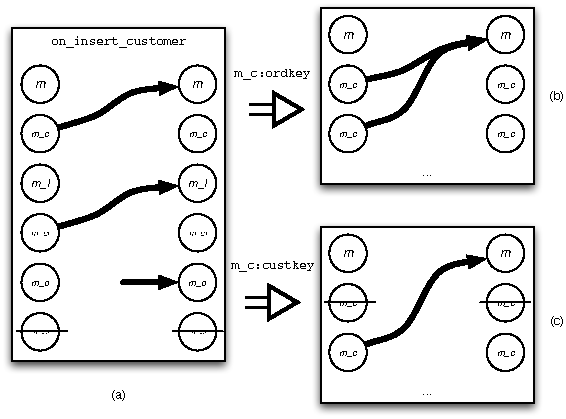
\includegraphics[width=2.5in]{graphics/MessagingGraph}
\end{center}
\caption{An example of a messaging graph based on Section \ref{sec:dbtoaster}'s example query.  (a) The messaging graph for the \texttt{on\_insert\_customer} event.  (b) The effects of splitting view $m_c$ on \texttt{ordkey}.  (c) The effects of splitting $m_c$ on \texttt{custkey}.}
\label{fig:diag:messagingGraph}
\vspace*{-0.2in}
\end{figure}

For example, consider the transition function that results from an update to the customer table.  One specific subtask of this transition reads $m_c$ and writes to $m$.  Treating each view as a node, this task has one edge with one read node and one write node.  

We consider database layout in terms of how we distribute, or partition it across a physical medium (i.e., memory, disk pages, or a cluster).  Viewed through the messaging graph, a partitioning is an assignment of all nodes in the graph to one (or more, in the case of replication) partition.  For example, if they were small enough, $m$ and $m_c$ might be placed on one disk page each.  Thus, the subtask requires a read on one page, and an update to a second.

Subdivision of individual views is represented in the messaging graph by splitting of graph nodes.  Of particular interest is how the new nodes interact with the hyperedge(s) connected to the original node.  As the split occurs, a node may stay connected to a hyperedge, the hyperedge may likewise be split, or in some cases, only one node will remain connected (see Figure \ref{fig:diag:messagingGraph}b,c).  We can exploit the limited range of node split/hyperedge interactions to select an effective partitioning scheme.

For example, when partitioning $m_c$, horizontal partitioning on the value of \texttt{ordkey} increases the number of nodes connected to the \texttt{on\_insert\_customer} task edge, while using \texttt{custkey} does not provoke an increase.  If we split the data represented by these nodes across multiple disks or servers, the computation must still access all of them.  The roles are reversed for the \texttt{on\_insert\_order} task edge.  Under (the false) assumption that both insert events occur with identical frequency, we can partition on both keys to minimize the number of connected nodes.

Additional knowledge about the dataset enhances the messaging graph.  For instance, the E-R diagram can be integrated into the messaging graph; the chain of foreign key dependencies in $q$ is strictly hierarchical.  We can use this information to maintain four partitions along a single axis with a secondary index to reduce the number of partitions accessed by either subtask.  This information can also be used to select a partitioning scheme that places often connected nodes into a single partition, analogous to co-clustering in a traditional DBMS.
